\documentclass[a4paper,11pt]{scrreprt}
% \usepackage{ngerman}
\usepackage[ngerman]{babel}
\usepackage[utf8x]{inputenc}
\usepackage[T1]{fontenc}
\usepackage{multicol}
\usepackage{ifpdf}
\usepackage[pdftex]{color}
\usepackage{scrhack}
\usepackage{listings}
\usepackage[colorlinks=true,linkcolor=black]{hyperref}
\usepackage{geometry}
\geometry{a4paper,left=30mm,right=20mm, top=26mm, bottom=35mm}
\usepackage{enumerate}

\ifpdf
  \usepackage[pdftex]{graphicx}
\else
  \usepackage[dvips]{graphicx}\fi

\newcommand{\kur}{\textit}
\newcommand{\ul}{\underline}
\newcommand{\bo}{\textbf}

\setcounter{tocdepth}{3}

\newcommand{\format}{\textbf}

\begin{document}

\begin{titlepage}

\vspace*{\fill}
  \begin{center}

\huge \bfseries AUTOSAR \\[2.5cm]

\textsc{\Large SoSe 2015}\\[0.5cm]

\large \today

\vfill

  \end{center}
\end{titlepage}

\begin{itemize}
\item[] \textbf{\large Beitragende:}\\
Daniel Tatzel (DT)\\
Florian Laufenböck (FL)\\
Markus Wildgruber (MW)\\
Philipp Eidenschink (PE)\\
Tim Schmiedl (TimS)\\
Tobias Schwindl (TobiS)
\end{itemize}

\bigskip

\begin{table}[!h]
 	\centering
	\begin{tabular}{|c|c|c|c|}
	\hline
	\textbf{VersionsNr} &  \textbf{Datum} & \textbf{Auslöser} & \textbf{Beschreibung} \\
	\hline
	1.0 & 21.04.2015 & DT & Erster Entwurf \\
	\hline
	\end{tabular}

% \caption{Überarbeitungshistorie}
\end{table}



\chapter{Projekt Beschreibung}

\section{Vernetzte Ballschussanlage}

\begin{itemize}
 \item 1-2 Bricks
 \item Ausgabe(durch Display,LEDs etc.)
 \item Stop-Trigger
 \item Variable Aufteilung unter den Bricks: Stopp-Taste, Auslösung Taste(auch über Ultraschall), Ausgabe
\end{itemize}

\section{Benötigte VFB-Komponenten und Schnittstellen (DT)}

\begin{itemize}
 \item Komponenten
 \begin{itemize}
  \item Application Software Component
  \item Sensor-Actuator Software Component
  \item ECU Abstraction Software Component
 \end{itemize}

 \item Schnittstellen
 \begin{itemize}
  \item Client/Server
  \item Events
  \item Sender/Receiver (auch mit synchronisierung)
 \end{itemize}

\end{itemize}


\section{Namenskonventionen und Standardrückgabtyp (Alle)}

\begin{tabular}{ll}
 Für RTE-Funktionen: & RTE\_<Funktionsname>\_<Portname>\_<Direction> \\
 Für den Rest: & <Komponente>\_<Funktionsname> \\
 \\
 Standardrückgabtyp: & uint32\_t \\
\end{tabular}

\begin{figure}[htbp]
 \centering
 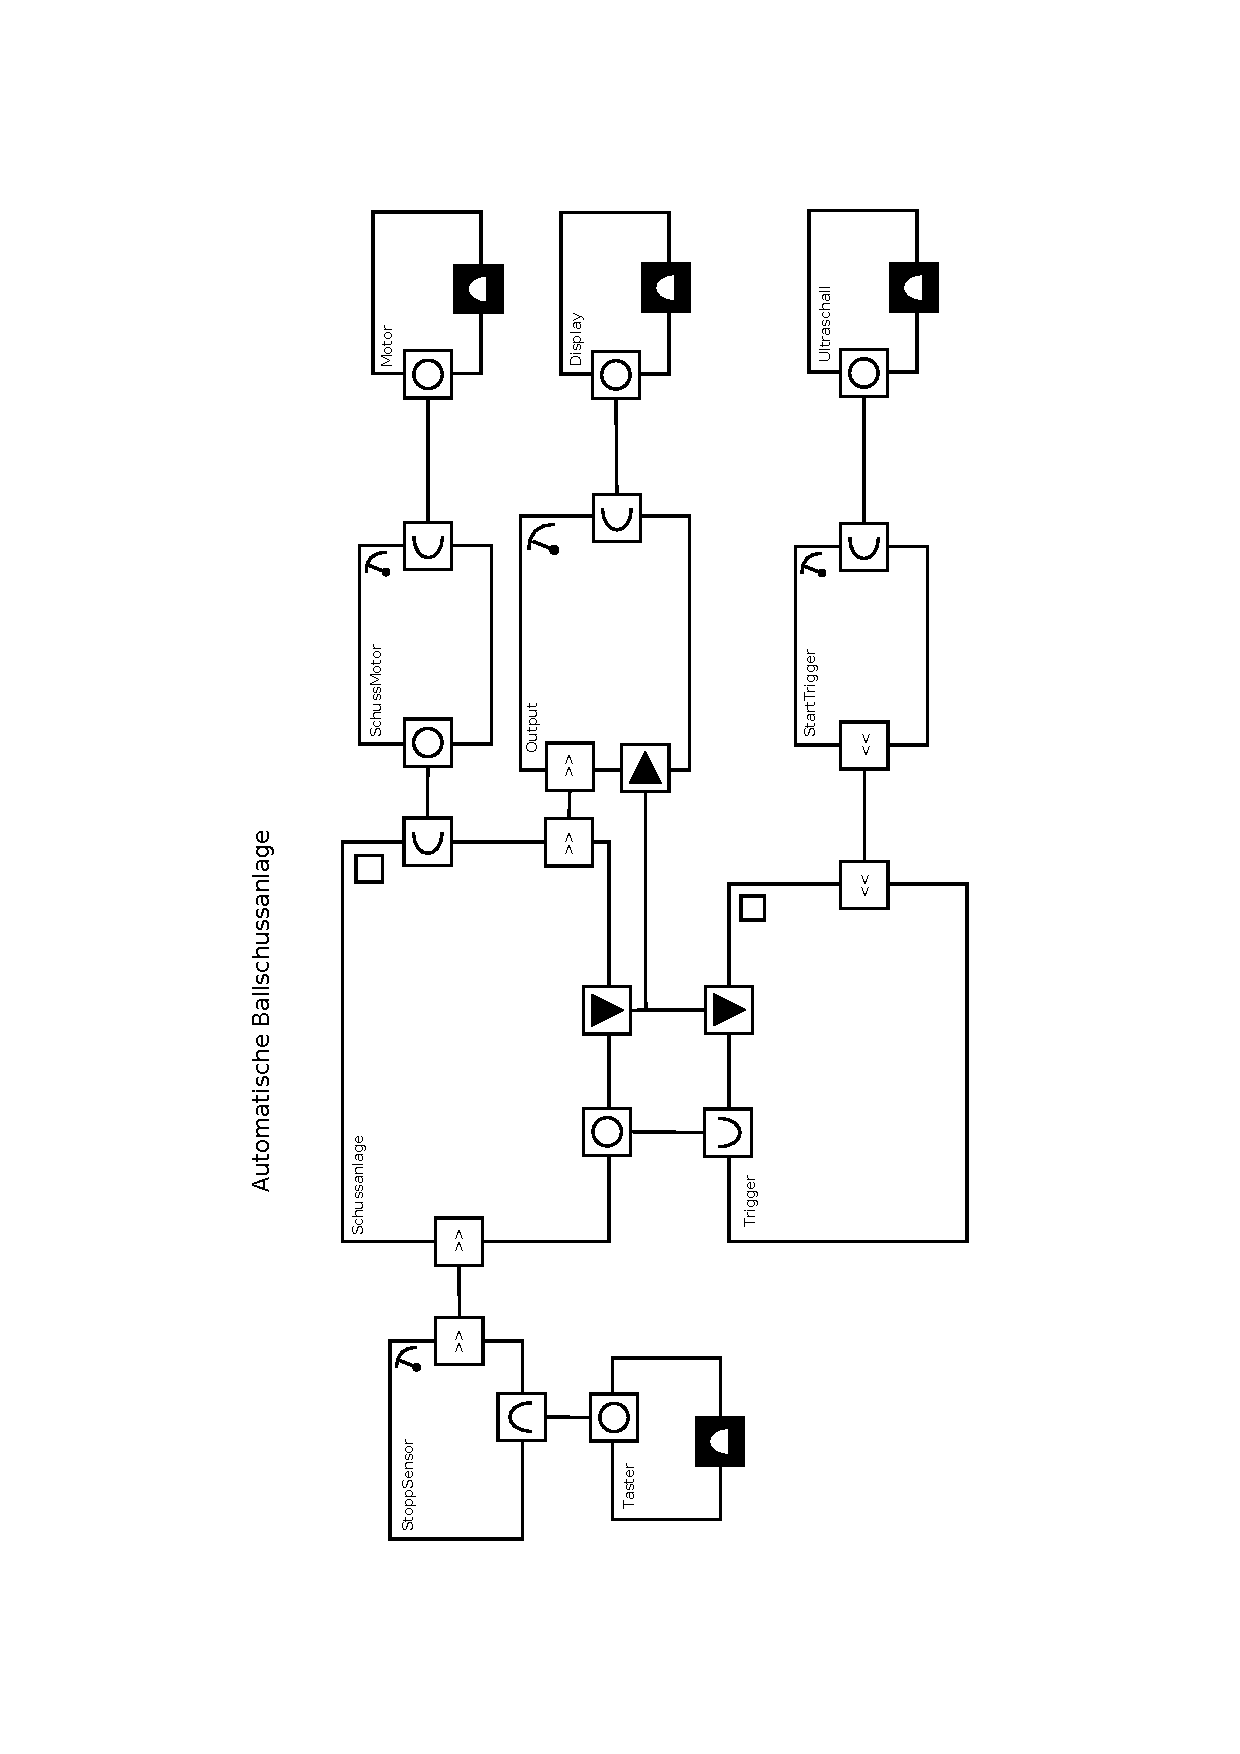
\includegraphics[scale=.75]{./KomponentenDiagramm.pdf}
 \label{fig:komponentendiag}
 \caption{Komponentendiagramm der Ballschussanlage (DT)}
\end{figure}

\chapter{Komponenten-Beschreibung}

\subsection*{Schussanlage (FL)}

\begin{itemize}
	\item Besteht aus einer Task mit zwei Runnables
	\item erste Runnable prüft periodische die Abbruchbedinung(hier: Taster)
	\item zweite Runnable managt den Schussmotor
	\item Kein Autostart des Tasks, wird über den Trigger gestartet
	\item Ports siehe Komponentendiagramm
\end{itemize}

Benötigt: Task und Event

\subsection*{Trigger (PE)}

\begin{itemize}
 \item Ein Task
 \item Wird zu beginn gestartet (Autostart)
 \item Wartet auf Event vom Input
\end{itemize}

Benötigt: Task und Event

\subsection*{Output (MW)}

\begin{itemize}
 \item Autostart
 \item Wird durch Event von Schussanlage getriggert
 \item Prüft nach Event die empfangene Nachricht
 \item Zeigt Nachricht in Abhängigkeit der empfangen Nachricht an
\end{itemize}

Benötigt: Task und Event


\subsection*{SchussMotor (TimS)}

\begin{itemize}
 \item Kein Autostart
 \item Servertask wird durch Schussanlage (client) gestartet
 \item Steuert Motor zum schießen an
\end{itemize}


\subsection*{StopSensor (TobiS)}

\begin{itemize}
 \item Autostart
 \item Prüft Taster
 \item Setzt Event für Schussanlage
\end{itemize}

Benötigt: Task, Timer und Event


\subsection*{StartTrigger (TobiS)}

\begin{itemize}
 \item Task zum Erkennen von Zielen
 \item Autostart
 \item Sendet Event an Trigger
 \item Erkennung durch periodische Abfrage
\end{itemize}

Benötigt: Task und Timer

\section{Architekturschicht und Funktionsapi}

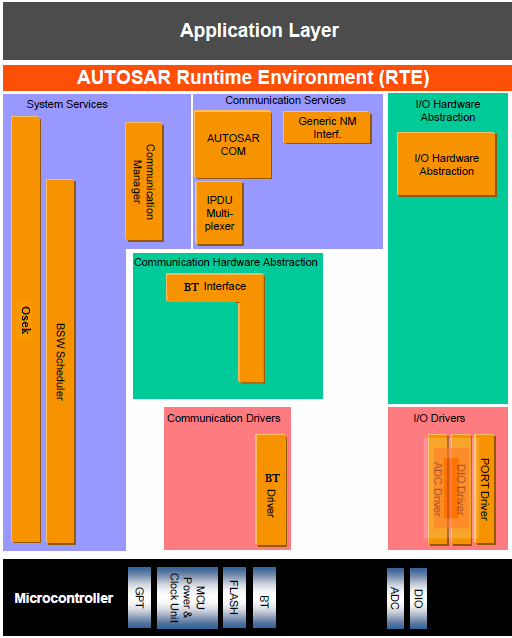
\includegraphics{Komponenten.png}

\subsection{Funktionapi}
\begin{enumerate}[1.)]
\item System Services\\
	keine Funktionen
\item Communication Services
	\begin{itemize}
	\item \underline{Abstraktionsebene um Nachrichten zu verschicken}
	\item \lstinline|StdReturnType TransmitMessage(char* message)|
	\item \lstinline|StdReturnType ReceiveMessage(char* message)|
	\end{itemize}
\item I/O Hardware Abstraction
	\begin{itemize}
	\item \lstinline|StdReturnType ReadDigitalInput(PortName)|
	\item \lstinline|StdReturnType ReadAnalogInput(PortName)|
	\item \lstinline|StdReturnType DriveMotor(Port_Name, Direction, speed, angle)|
	\end{itemize}
\item Communication Hardware Abstraction
	\begin{itemize}
	\item \underline{Für unser Projekt eigentlich unnötig, da wir nur eine Kommunikationsebene haben}(theoretisch mehr durch I2C, aber hier uninteressant)
	\item \lstinline|StdReturnType SendMessageBT(char* message )|
	\item \lstinline|StdReturnType GetMessageBT(char* message)|
	\end{itemize}
\item Communication Drivers
	\begin{itemize}
	\item \underline{es wird nur ein Treiber für das Hardware BT gebraucht:}
	\item \lstinline|StdReturnType BT_Write(char* message)| 
	\item \lstinline|StdReturnType BT_Read(char* message)|
	\end{itemize}
\item I/O Drivers
	\begin{itemize}
	\item \underline{benötigt für den zusätzlichen I2C expander}
	\item \lstinline|StdReturnType ReadI2C(PortName)|
	\item \lstinline|StdReturnType WriteI2C(PortName)|	
	\end{itemize}
\end{enumerate}
\end{document}

